\section{Model Structure}

- detail the structure of the model, eg. the training was called in a notebook (main.ipynb) but the training and the model was defined in discrete python files of their own in accordance with modularity best practices.

\subsection{Model Structure}

The model is a convolutional neural network (CNN) designed for binary image classification. It accepts full-size images of shape $(512, 512, 3)$.

Input $(512\times 512\times 3)$ $\rightarrow$ \texttt{Rescaling}(1/255) $\rightarrow$ 
\texttt{Conv2D}($f_1$, $3{\times}3$, ReLU) $\rightarrow$ \texttt{Pool} (max/avg) $\rightarrow$
\texttt{Conv2D}($f_2$, $3{\times}3$, ReLU) $\rightarrow$ \texttt{Pool} (max/avg) $\rightarrow$
Global (max/avg) pooling $\rightarrow$ \texttt{Flatten} $\rightarrow$
\texttt{Dense}($d$, ReLU) $\rightarrow$ optional \texttt{Dropout}($p$) $\rightarrow$
\texttt{Dense}(1, sigmoid). Trained with binary cross-entropy and \texttt{adam}/\texttt{adagrad}.

Adam was chosen as one of the considered optimisers, as it is known to converge rapidly, and rectifies vanishing learning rate and high variance, therefore being the most popular optimiser \cite{RAIAAN2024100470}

Adagrad was chosen as the second potential optimiser, as the learning rate would not need manual tuning, and is known to perform better than alternatives like SGD, MBGD, and primitive momentum based optimisers. Though it should be noted that it has the weakness of a constantly decreasing learning rate, resulting in slower convergence \cite{RAIAAN2024100470}

\note{mention that the most optimal loss function for binary classification task is binary cross entropy.}

\note{mention the fact that i trained on 3 epochs}

\subsection{Hyperparameter Tuning with Hyperband}

Hyperparameter tuning was performed to maximise the models performance through iteration of most of its parameters. 

\Cref{tab:tunable_hyperparameters} shows a list of the parameters being tuned in the above model. It is evident that this is a very large parameter space, and it is therefore not feasible to find the best possible hyperparamet.

\begin{figure}[p]
\lstinputlisting[language=Python, caption=Hyperparameter tuning code extracts from \code{main.ipynb} and \code{src/train.py}, label=code:hyperparameter_tuning]{code_chunks/sec_3_hp_tuning.py}
\end{figure}


The Hyperband algorithm is used for hyperparameter optimization. Hyperband eliminates poorly performing hyperparameter combinations and focuses on promising ones, thus saving computational time compared to other methods like Bayesian optimization and grid search. 

\begin{table}[h]
\centering
\caption{Tunable Hyperparameters and Final Chosen Values}
\begin{tabular}{lll}
\toprule
\textbf{Hyperparameter} & \textbf{Range/Choices} & \textbf{Final Value} \\
\midrule
learning rate           & $1{\times}10^{-4}$ to $1{\times}10^{-2}$ (log scale) & 0.00149 \\
dropout-rate            & $0.0$ to $0.5$ (used if \texttt{use-dropout=true}) & 0.284 \\
conv1-filters ($f_1$)   & $16$ to $128$ & 24 \\
conv2-filters ($f_2$)   & $32$ to $256$ & 107 \\
dense-units ($d$)       & $64$ to $512$ & 254 \\
pooling                 & \texttt{max}, \texttt{avg} & max \\
use-dropout             & \texttt{true}, \texttt{false} & true \\
optimizer               & \texttt{adam}, \texttt{adagrad} & adam \\
\bottomrule
\end{tabular}
\label{tab:tunable_hyperparameters}
\end{table}


\section{Model Deployment} \label{sec:model_deployment}


\begin{figure}[h]
    \centering
    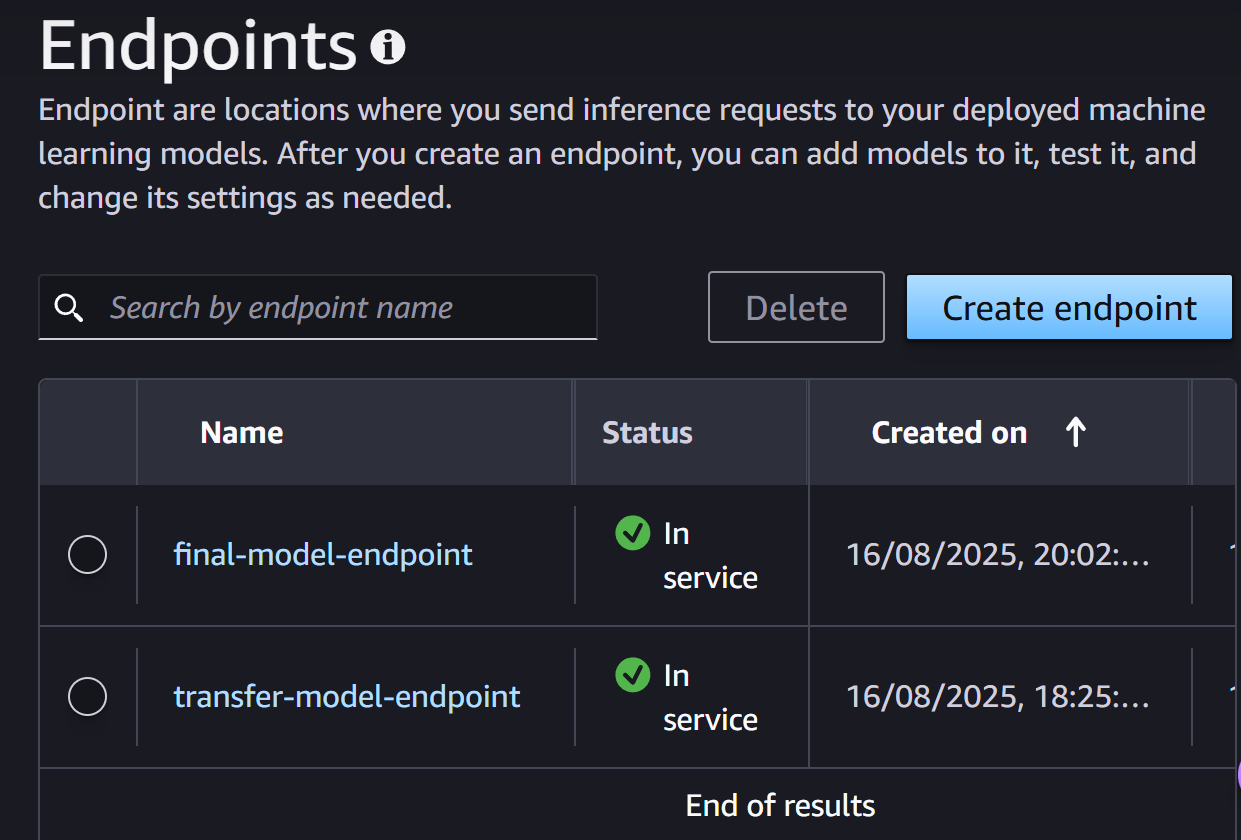
\includegraphics[width=200px]{figures/endpoints_screenshot.png} % Image filename
    \centering
    \caption{Endpoint page screenshot in Sagemaker, as evidence of deployment} % Caption
    \label{fig:endpoint} % Label
\end{figure}

The best hyperparameters found on the smaller training set were then extracted, and trained on the larger dataset. This 

\section{Transfer Learning}

The list of the possible CNN structures available for use for transfer learning can be seen in \cite{keras_applications}. Of these, EfficientNetV2 was selected as the most suitable architecture due to its demonstrated balance between accuracy and computational efficiency on general image classification tasks. This makes it well-suited for the diverse and varied images present in the aiornot dataset \cite{keras_applications, tan2021efficientnetv2}.

Using an endpoint, the model was then evaluated on its precision, recall, f1 score, and accuracy. \Cref{fig:endpoint} shows the endpoint configuration in Sagemaker. This allowed for evaluation of the models performance, whilst not being limited by the RAM limitations of the notebook environent in Sagemaker studio. 

Deploying the transfer learning model, again using a sagemaker endpoint allowed a comparison between both models on the holdout set.

\section{Model Comparison And Evaluation}

In this section, we compare the performance of the different models trained on the dataset. Evaluation metrics were calculated by invoking the model endpoints on the holdout set, which was not used during training or validation. This ensures that the models' performance is on unseen data, better modelling a general use case.

The endpoints were deployed as real time endpoints, operating on a server and interacting through the user with a HTTP request. While this does mean they can be accessed at any time by any user who has the appropriate permissions, it also means that the network requests are limited to \note{X Mb}, which equates to only 4 500x500 rgb images at a time, making the evaluation process slower. It was for this reason that the holdout set was limited to only 500 images.

\begin{table}[h]
\centering
\caption{Model Comparison}
\begin{tabular}{lcccc}
\toprule
\textbf{Model} & \textbf{Accuracy} & \textbf{Precision} & \textbf{Recall} & \textbf{F1 Score} \\
\midrule
Main Model     & 0.854          & 0.833          & \textbf{0.906} & \textbf{0.868} \\
Transfer Model & \textbf{0.856} & \textbf{0.875} & 0.849 & 0.862 \\
\midrule
Difference & 0.002 & 0.042 & 0.057 & 0.006 \\
\bottomrule
\end{tabular}
\label{tab:model_comparison}
\end{table}

\begin{figure}[h]
    \centering
    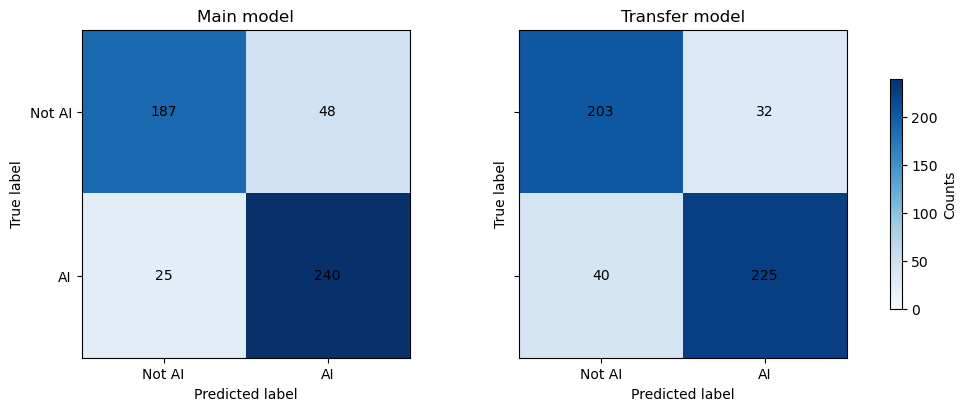
\includegraphics[width=0.9\linewidth]{figures/confusion_matrix.png} % Image filename
    \centering
    \caption{Confusion Matrix of main model and transfer learning model} % Caption
    \label{fig:confusion_matrixes} % Label
\end{figure}

The results of the model evaluation are summarized in \Cref{tab:model_comparison}. The table highlights the key performance indicators for each model. It can be seen that the EfficientNet transfer learning model and the main model have very comparable performance - with the EfficientNet model and main model achieving an accuracy of 85.6\% and 85.4\% respectively - a difference of only 0.2\%. Furthermore the EfficientNet and main model achieved F1 scores of 0.862 and 0.868 respectively, a difference of only 0.006.

Where these models differ is their precision and recall. The EfficientNet model achieved a precision of 87.5\% (4.2\% higher than the main models 83.3\%.) The main model achieved a recall of 90.6\% (5.7\% higher than the EfficientNet models 84.9\%.) This means that the EfficientNet model is better at minimising false positive AI detection, whereas the main model is better at detecting AI cases without missing them (i.e. reducing false negatives). 

This is evident in \cref{fig:confusion_matrixes}, where the EfficientNet model has 32 false posiives compared to the main models 48. Similarly, the main model has only 25 false negatives, compared to the EfficientNet models 40.

\section{AWS Sagemaker Information and Discussion}

This project was developed using AWS Sagemaker. \Cref{fig:aws_cost_summary}, which overall was less than \$15. This was achieved due to careful management of resources with a known budget of \$50 leading to selection of smaller instance types (using general purpose ml.c5.2xlarge instances for training and inference rather than larger, more expensive GPU instances). This of course, came at the cost of longer training times, but was deemed acceptable given the budget constraints, and the fact that the workflow would be very easily extensible to a more expensive configuration in a real world deployment scenario.

\begin{figure}[h]
    \centering
    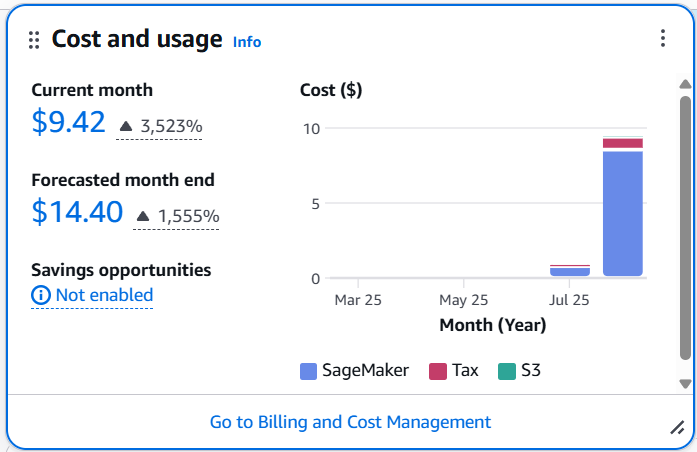
\includegraphics[width=300px]{figures/aws_cost_summary.png} % Image filename
    \centering
    \caption{Project Cost summary} % Caption
    \label{fig:aws_cost_summary} % Label
\end{figure}


\note{mention the drawbacks of the deployment here, though have the code chunk (with the creation of the endpoint and the prediction extraction, (and in the appendix have the code snippets for the table and the confusion matrix))}


\section{Final Model Discussion and Conclusion}

This report proposed two models to detect if an image is generated using ai - one model developed through hyperparameter tuning, and the other through transfer learning from EfficientNet. The results indicate that both models perform comparably, with slight differences in precision and recall.

The original research objective was to make a tool to distinguish between AI-generated and real images, ultimately as a means to identify the spread of misinformation and other harms in online discourse. Were this model to be deployed as a 'first step' with the intention of more thoughrough investigation, it would be more beneficial to be relaxed on false positives, and minimise false negatives, given the false positives would be vindicated with further analysis or research.

It is for this reason that, assuming this approach, the main model would be the preferred model, as it has a higher recall (90.6\% vs 84.9\%) and therefore is slightly better at detecting AI-generated images without missing them. \note{talk about the paper at the start and that we didnt achieve research level performance, nor the experience to use the dataset they made}

\note{mention the limitation of fixed resolutions/aspect ratio of 1:1}

Overall it can be concluded that the models developed in this investigation are effective at distinguising AI-generated images from other images, successfully training and deploying 2 models to make this prediction. 
